To evaluate the proposed string and fret classifier along  with the plucking position estimator some experiments have been conducted as described next. These experiments focus on comparing the proposed simulation method to~\cite{hjerrild::icassp19}. This is done with segment-by-segment estimation and classification using short 40 ms segments as this enables high-tempo and real-time applications. Hence, the experiments aim to demonstrate that this it is possible to classify string and fret from a simulated feature space, and to which extend both methods are robust to noise.
The classification of the string and fret is tested on recordings of two guitars from~\cite{hjerrild::icassp19}. The data and MATLAB code is available online\footnote{\url{https://tinyurl.com/waspaa2019}} and we refer to the available code for implementation details. All signals have been induced with additive white Gaussian noise (AWGN) at various levels of average signal to noise ratio (SNR). The class dependent model of the classifier is trained from simulated feature distributions, thus all string and fret combinations is purely based on physical properties. The resulting distributions are shown in Figure~\ref{fig:string_and_fret_model}. The state-of-the-art comparison~\cite{hjerrild::icassp19} is trained on 60 recordings obtained from the 12th fret on all six strings. A plausibility filter~\cite{abesser:automatic_string_detection_ml,hjerrild::icassp19} based on the equal tempered scale was applied to both string and fret classifiers and the resulting error rates are shown in Figure~\ref{fig:string_fret_electric} as a function of SNR. %In Figure.~\ref{tbl:str_confusion_firebrand} are shown here for the strings, and we observe that %the acoustic guitar has a very low error rate while for the electric guitar it is on average $3\%$. The biggest confusion occurs between strings 3 and 4. We have observed that the amplitudes for $m\!\!\gg\!\!1$ of the acoustic guitar has much more energy than the electric guitar, which could explain the difference in accuracy as being related to acoustic qualities of the guitar and pickup~\cite{fletcher:physics_of_musical_instruments}.  
%
\begin{figure}[t]
\centering
   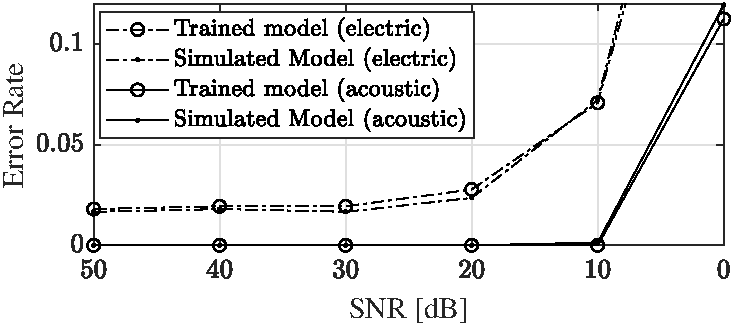
\includegraphics[width=.86\linewidth]{img/SNRfig_both.pdf}\vspace{-2mm}
   \caption{String, fret classification error rates as a function of SNR. Each marker represents 720 classifications. The trained model represents~\cite{hjerrild::icassp19} and the simulated model represents the proposed method.}
   \label{fig:string_fret_electric} 
\end{figure}
%
%
%
\begin{figure}[t]
\centering
   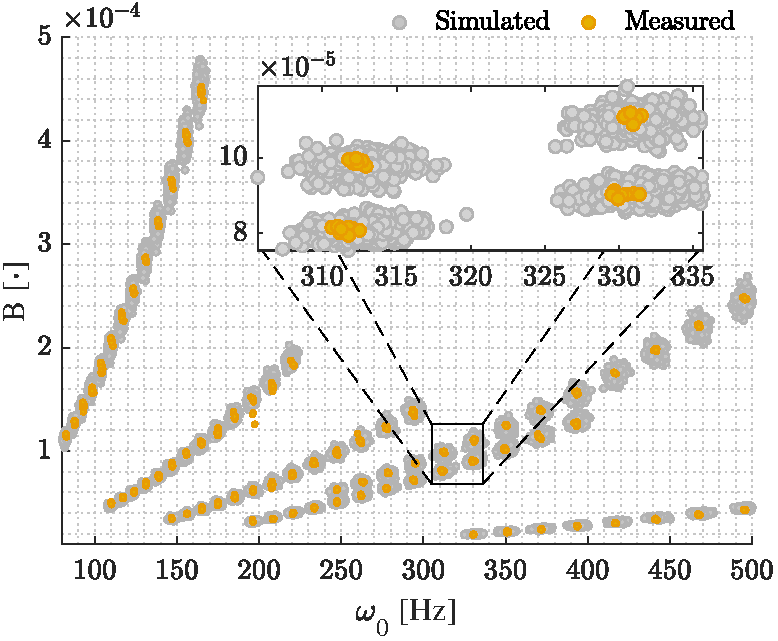
\includegraphics[width=.96\linewidth]{img/w0_vs_B2.pdf}\vspace{-2mm}
   \caption{Comparison of simulated random variables to the measured estimates of the features for the acoustic guitar. For each class there is 500 simulated values and 10 estimated measurements.}
   \label{fig:string_and_fret_model} 
\end{figure}


\begin{figure}[t]
\centering
% \begin{subfigure}
   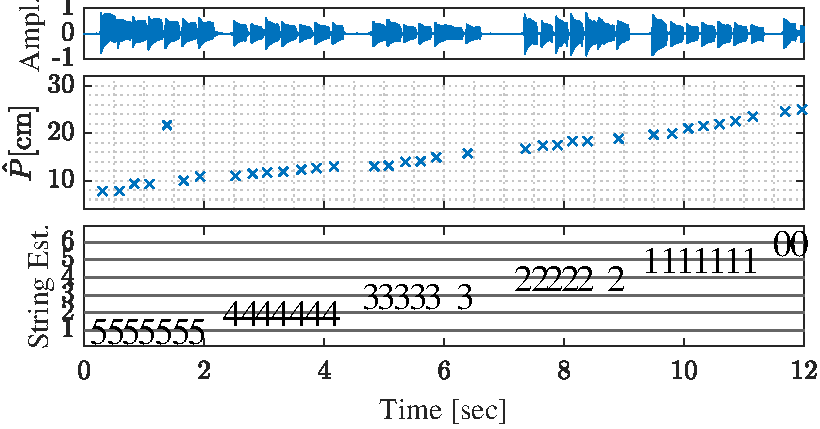
\includegraphics[width=.86\linewidth]{img/tablature_constant_note25_LSD}\vspace{-2mm}
   \caption{String, fret and plucking position estimates with moving plucking position and moving string and fret for electric guitar.}
   \label{fig:pluck_position_fixed_tabs} 
% \end{subfigure}
% \vspace{4mm}
% \begin{subfigure}
%   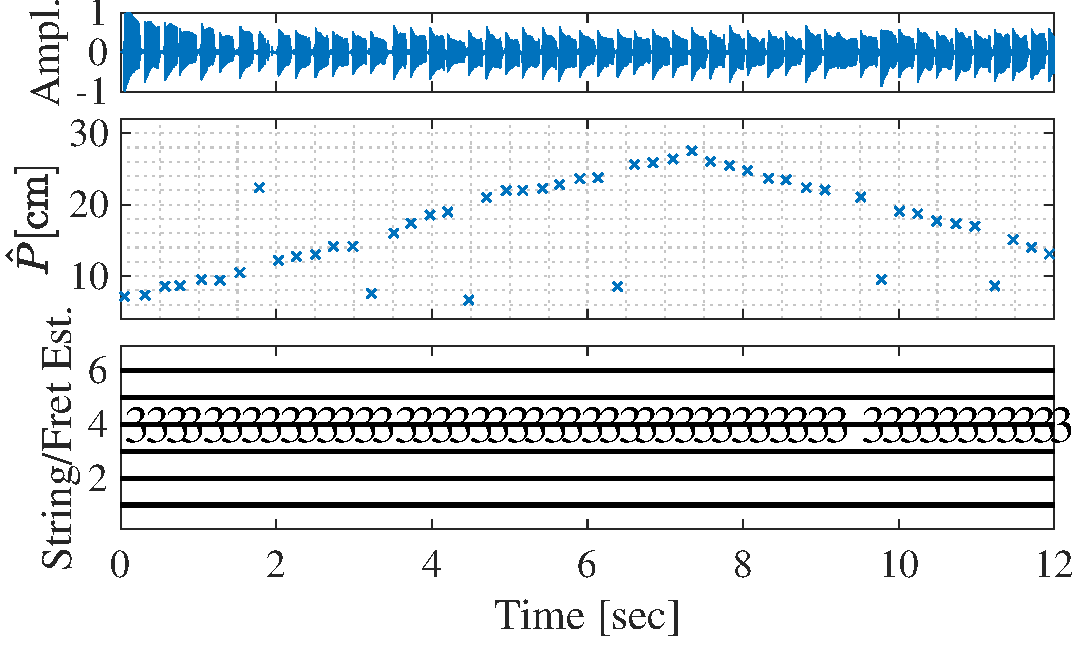
\includegraphics[width=.95\linewidth]{img/tablature_constant_note8}\vspace{-2mm}
%   \caption{String, fret and plucking position estimates with moving plucking position and moving string and fret for electric guitar.}
%   \label{fig:pluck_position_varied_tabs}
% \end{subfigure}
\end{figure}